\documentclass{standalone}
\usepackage{tikz}
\usetikzlibrary{bayesnet}

\begin{document}
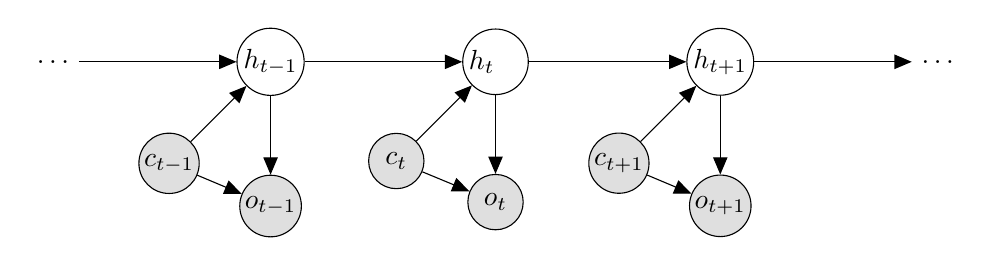
\begin{tikzpicture}
    \node[latent] (htm1) {$h_{t-1}$} ;
    \node[obs, below = of htm1] (otm1) {$o_{t-1}$} ;
    \node[obs, below left = of htm1] (ctm1) {$c_{t-1}$} ;
    \edge {htm1} {otm1} ;
    \edge {ctm1} {otm1,htm1} ;

    \node[latent, right = 2cm of htm1] (ht) {$h_{t\quad}$} ;
    \node[obs, below = of ht] (ot) {$o_t$} ;
    \node[obs, below left = of ht] (ct) {$c_t$} ;
    \edge {ht} {ot} ;
    \edge {ct} {ot,ht} ;

    \node[latent, right = 2cm of ht] (ht1) {$h_{t+1}$} ;
    \node[obs, below = of ht1] (ot1) {$o_{t+1}$} ;
    \node[obs, below left = of ht1] (ct1) {$c_{t+1}$} ;
    \edge {ht1} {ot1} ;
    \edge {ct1} {ot1,ht1} ;

    \edge {htm1} {ht} ;
    \edge {ht} {ht1} ;

    \node[right = 2cm of ht1] (ellipsesR) {$\ldots$} ;
    \node[left = 2cm of htm1] (ellipsesL) {$\ldots$} ;
    \edge {ellipsesL} {htm1} ;
    \edge {ht1} {ellipsesR} ;
\end{tikzpicture}
\end{document}
